
  
\documentclass[journal,12pt,twocolumn]{IEEEtran}

\usepackage{setspace}
\usepackage{gensymb}
\singlespacing
\usepackage[cmex10]{amsmath}

\usepackage{amsthm}

\usepackage{mathrsfs}
\usepackage{txfonts}
\usepackage{stfloats}
\usepackage{bm}
\usepackage{cite}
\usepackage{cases}
\usepackage{subfig}

\usepackage{longtable}
\usepackage{multirow}

\usepackage{enumitem}
\usepackage{mathtools}
\usepackage{steinmetz}
\usepackage{tikz}
\usepackage{circuitikz}
\usepackage{verbatim}
\usepackage{tfrupee}
\usepackage[breaklinks=true]{hyperref}
\usepackage{graphicx}
\usepackage{tkz-euclide}

\usetikzlibrary{calc,math}
\usepackage{listings}
    \usepackage{color}                                            %%
    \usepackage{array}                                            %%
    \usepackage{longtable}                                        %%
    \usepackage{calc}                                             %%
    \usepackage{multirow}                                         %%
    \usepackage{hhline}                                           %%
    \usepackage{ifthen}                                           %%
    \usepackage{lscape}     
\usepackage{multicol}
\usepackage{chngcntr}

\DeclareMathOperator*{\Res}{Res}

\renewcommand\thesection{\arabic{section}}
\renewcommand\thesubsection{\thesection.\arabic{subsection}}
\renewcommand\thesubsubsection{\thesubsection.\arabic{subsubsection}}

\renewcommand\thesectiondis{\arabic{section}}
\renewcommand\thesubsectiondis{\thesectiondis.\arabic{subsection}}
\renewcommand\thesubsubsectiondis{\thesubsectiondis.\arabic{subsubsection}}


\hyphenation{op-tical net-works semi-conduc-tor}
\def\inputGnumericTable{}                                 %%

\lstset{
%language=C,
frame=single, 
breaklines=true,
columns=fullflexible
}
\begin{document}

\newcommand{\BEQA}{\begin{eqnarray}}
\newcommand{\EEQA}{\end{eqnarray}}
\newcommand{\define}{\stackrel{\triangle}{=}}
\bibliographystyle{IEEEtran}
\raggedbottom
\setlength{\parindent}{0pt}
\providecommand{\mbf}{\mathbf}
\providecommand{\pr}[1]{\ensuremath{\Pr\left(#1\right)}}
\providecommand{\qfunc}[1]{\ensuremath{Q\left(#1\right)}}
\providecommand{\sbrak}[1]{\ensuremath{{}\left[#1\right]}}
\providecommand{\lsbrak}[1]{\ensuremath{{}\left[#1\right.}}
\providecommand{\rsbrak}[1]{\ensuremath{{}\left.#1\right]}}
\providecommand{\brak}[1]{\ensuremath{\left(#1\right)}}
\providecommand{\lbrak}[1]{\ensuremath{\left(#1\right.}}
\providecommand{\rbrak}[1]{\ensuremath{\left.#1\right)}}
\providecommand{\cbrak}[1]{\ensuremath{\left\{#1\right\}}}
\providecommand{\lcbrak}[1]{\ensuremath{\left\{#1\right.}}
\providecommand{\rcbrak}[1]{\ensuremath{\left.#1\right\}}}
\theoremstyle{remark}
\newtheorem{rem}{Remark}
\newcommand{\sgn}{\mathop{\mathrm{sgn}}}
\providecommand{\abs}[1]{\vert#1\vert}
\providecommand{\res}[1]{\Res\displaylimits_{#1}} 
\providecommand{\norm}[1]{\lVert#1\rVert}
%\providecommand{\norm}[1]{\lVert#1\rVert}
\providecommand{\mtx}[1]{\mathbf{#1}}
\providecommand{\mean}[1]{E[ #1 ]}
\providecommand{\fourier}{\overset{\mathcal{F}}{ \rightleftharpoons}}
%\providecommand{\hilbert}{\overset{\mathcal{H}}{ \rightleftharpoons}}
\providecommand{\system}{\overset{\mathcal{H}}{ \longleftrightarrow}}
	%\newcommand{\solution}[2]{\textbf{Solution:}{#1}}
\newcommand{\solution}{\noindent \textbf{Solution: }}
\newcommand{\cosec}{\,\text{cosec}\,}
\providecommand{\dec}[2]{\ensuremath{\overset{#1}{\underset{#2}{\gtrless}}}}
\newcommand{\myvec}[1]{\ensuremath{\begin{pmatrix}#1\end{pmatrix}}}
\newcommand{\mydet}[1]{\ensuremath{\begin{vmatrix}#1\end{vmatrix}}}
\numberwithin{equation}{subsection}
\makeatletter
\@addtoreset{figure}{problem}
\makeatother
\let\StandardTheFigure\thefigure
\let\vec\mathbf
\renewcommand{\thefigure}{\theproblem}
\def\putbox#1#2#3{\makebox[0in][l]{\makebox[#1][l]{}\raisebox{\baselineskip}[0in][0in]{\raisebox{#2}[0in][0in]{#3}}}}
     \def\rightbox#1{\makebox[0in][r]{#1}}
     \def\centbox#1{\makebox[0in]{#1}}
     \def\topbox#1{\raisebox{-\baselineskip}[0in][0in]{#1}}
     \def\midbox#1{\raisebox{-0.5\baselineskip}[0in][0in]{#1}}
\vspace{3cm}
\title{Assignment 7}
\author{Adarsh Sai - AI20BTECH11001}
\maketitle
\newpage
\bigskip
\renewcommand{\thefigure}{\theenumi}
\renewcommand{\thetable}{\theenumi}
Download all python codes from 
\begin{lstlisting}
https://github.com/Adarsh541/AI1103-prob-and-ranvar/blob/%main/Assignment6/codes/Assignment6.py
\end{lstlisting}
%
Download latex-tikz codes from 
%
\begin{lstlisting}
https://github.com/Adarsh541/AI1103-prob-and-ranvar/blob/main/Assignment7/Assignment7.tex
\end{lstlisting}
\section{Problem(CSIR UGC NET EXAM(June 2012)Q.112)}
Let $X_1,X_2,X_3,....,X_n$ be i.i.d observations from a distribution with continuous probability density function f which is symmetric around $\theta$ i.e
\begin{align}
    f\brak{x-\theta}=f\brak{\theta -x}
\end{align}
for all real x.Consider the test $H_0: \theta =0$ vs $H_1:  \theta >0$ and the sign test statistic
\begin{align}
    S_n = \sum_{i=1}^{n} sign(X_i)
\end{align}
where
\begin{align}
    sign(x) =
    \begin{cases}
    1  & x>0\\
    0  & x=0\\
    -1 & x<0
    \end{cases}
\end{align}
Let $z_\alpha$ be the upper $100(1-\alpha)^{th}$ percentile of the standard normal distribution where $0<\alpha <1$. Which of the following is/are correct?
\begin{enumerate}
    \item If $\theta =0$ then $ \lim_{n\to\infty} P\cbrak{S_n > \sqrt{n}z_{\alpha}} =1 $\\
    \item If $\theta =0$ then $ \lim_{n\to\infty} P\cbrak{S_n > \sqrt{n}z_{\alpha}} =\alpha $\\
    \item If $\theta >0$ then $ \lim_{n\to\infty} P\cbrak{S_n > \sqrt{n}z_{\alpha}} = 1 $\\
    \item If $\theta >0$ then $ \lim_{n\to\infty} P\cbrak{S_n > \sqrt{n}z_{\alpha}} =\alpha $
\end{enumerate}
\section{Solution(CSIR UGC NET EXAM(June 2012)Q.112)}
Assume hypothesis
$H_0:\theta=0$ is true.
\begin{enumerate}
\item Given X is symmetric around zero.
 \begin{align}
  f_X(x)&=f_X(-x)\\
  \int_{0}^{\infty}f_X(x)dx&=\int_{0}^{\infty}f_X(-x)dx
  \label{int}
\end{align}
\begin{enumerate}
\item Solving LHS of $\eqref{int}$
\begin{align}
    \int_{0}^{\infty}f_X(x)dx=\pr{X\geq0}
\end{align}
\item Solving RHS of $\eqref{int}$
\begin{align}
    \int_{0}^{\infty}f_X(-x)dx
\end{align}
Changing $-x \rightarrow x$ we get 
\begin{align}
  \int_{0}^{\infty}f_X(-x)dx&=\int_{-\infty}^{0}f_X(x)dx\label{rhs}\\
  &=\pr{X\leq0}
\end{align}
\end{enumerate}
but
\begin{align}
  \int_{-\infty}^{0}f_X(x)dx+\int_{0}^{\infty}f_X(x)dx=1
  \label{pr}
\end{align}
from $\eqref{int}$ , $\eqref{rhs}$ and $\eqref{pr}$
\begin{align}
\int_{-\infty}^{0}f_X(x)dx=\int_{0}^{\infty}f_X(x)dx=\frac{1}{2}
\end{align}
\begin{align}
    \implies \pr{X\leq 0}=\pr{X\geq0}=\frac{1}{2}
    \label{sym}
\end{align}
\item Let Y be a random variable such that
\begin{align}
    Y=sign(X)
\end{align}
\begin{align}
    Y=
    \begin{cases}
     1 & X>0\\
    -1 & X<0
    \end{cases}
    \label{t}
\end{align}
From $\eqref{sym}$ and $\eqref{t}$
we have
\begin{align}
   \pr{Y=-1}=\pr{Y=1}=\frac{1}{2} 
\end{align}
So $Y=sign(X)$ is also symmetric around zero.
\begin{figure}[!ht]
\centering
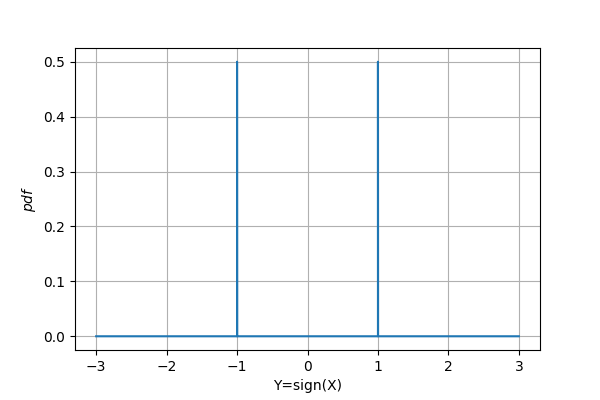
\includegraphics[width=\columnwidth]{Assignment7.png}
\caption{pdf of $ Y=sign(X)$}
\label{pdf}
\end{figure}
\begin{align}
   \implies \mu_y = 0 
\end{align}
and variance is
\begin{align}
    \sigma_y^2 &= (-1)^2\brak{\frac{1}{2}}+(1)^2\brak{\frac{1}{2}}\\
    &=1
\end{align}
\item Given
\begin{align}
    S_n&=\sum_{i=1}^{n} sign(X_i)\\
    S_n&=\sum_{i=1}^{n} Y_i
\end{align}
From central limit theorem 
\begin{align}
    Z&=\lim_{n\to\infty}\sqrt{n}\brak{\frac{\frac{S_n}{n}-\mu_y}{\sigma_y}}\\
    &=\lim_{n\to\infty}\sqrt{n}\brak{\frac{S_n}{n}}\\
    &=\lim_{n\to\infty}\brak{\frac{S_n}{\sqrt{n}}}
    \label{clt}
\end{align}
where Z is a standard normal variable N(0,1).
\begin{enumerate}
    \item Given
\begin{align}
    \alpha = P\cbrak{Z>z_\alpha}\label{uff}
\end{align}
So from $\eqref{clt}$ and $\eqref{uff}$
\begin{align}
\lim_{n\to\infty}P\cbrak{\frac{S_n}{\sqrt{n}}>z_\alpha}&=
\alpha\\
\implies \lim_{n\to\infty}P\cbrak{S_n>\sqrt{n}z_\alpha}&=
\alpha
\end{align}
\end{enumerate}
\end{enumerate}
\end{document}


